\subsection{Results of Experiments}
FR evaluation will be conducted on two different classifiers for the two
presented approaches respectively. In the case of PCA, a support vector machine
(SVM) is used for classification. The experiments have been conducted using
sci-kitlearn \cite{sk} library in Python. In the autoencoder's case, the
extracted features will be forwarded to a softmax classifier, consisting of one
fully-connected layer and softmax activation function with 38, accounting the
amount of classes. I have adapted Facebook DeepFace model implementation from
\cite{serengil2017tensorflow101}, which uses Keras \cite{gulli2017deep} and
Tensorflow \cite{tensorflow} as its backend.

\begin{figure}[h]
  \begin{subfigure}{}
    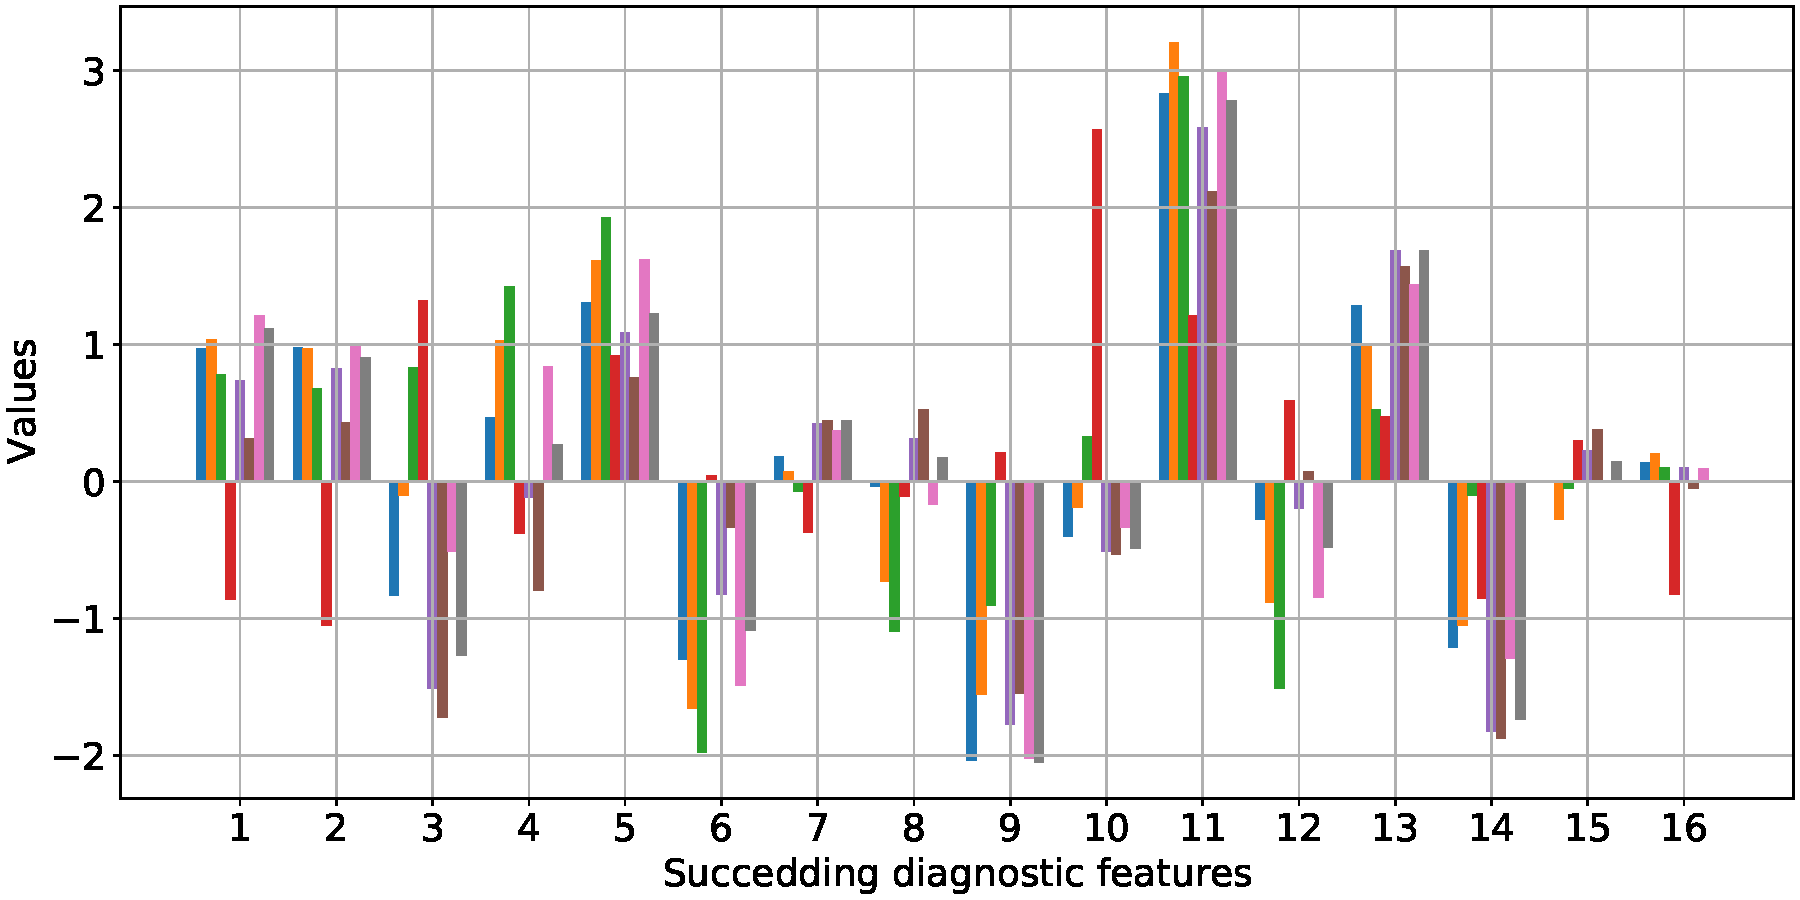
\includegraphics[width=\columnwidth]{PCAfeatures.pdf}
  \end{subfigure}

  \begin{subfigure}{}
    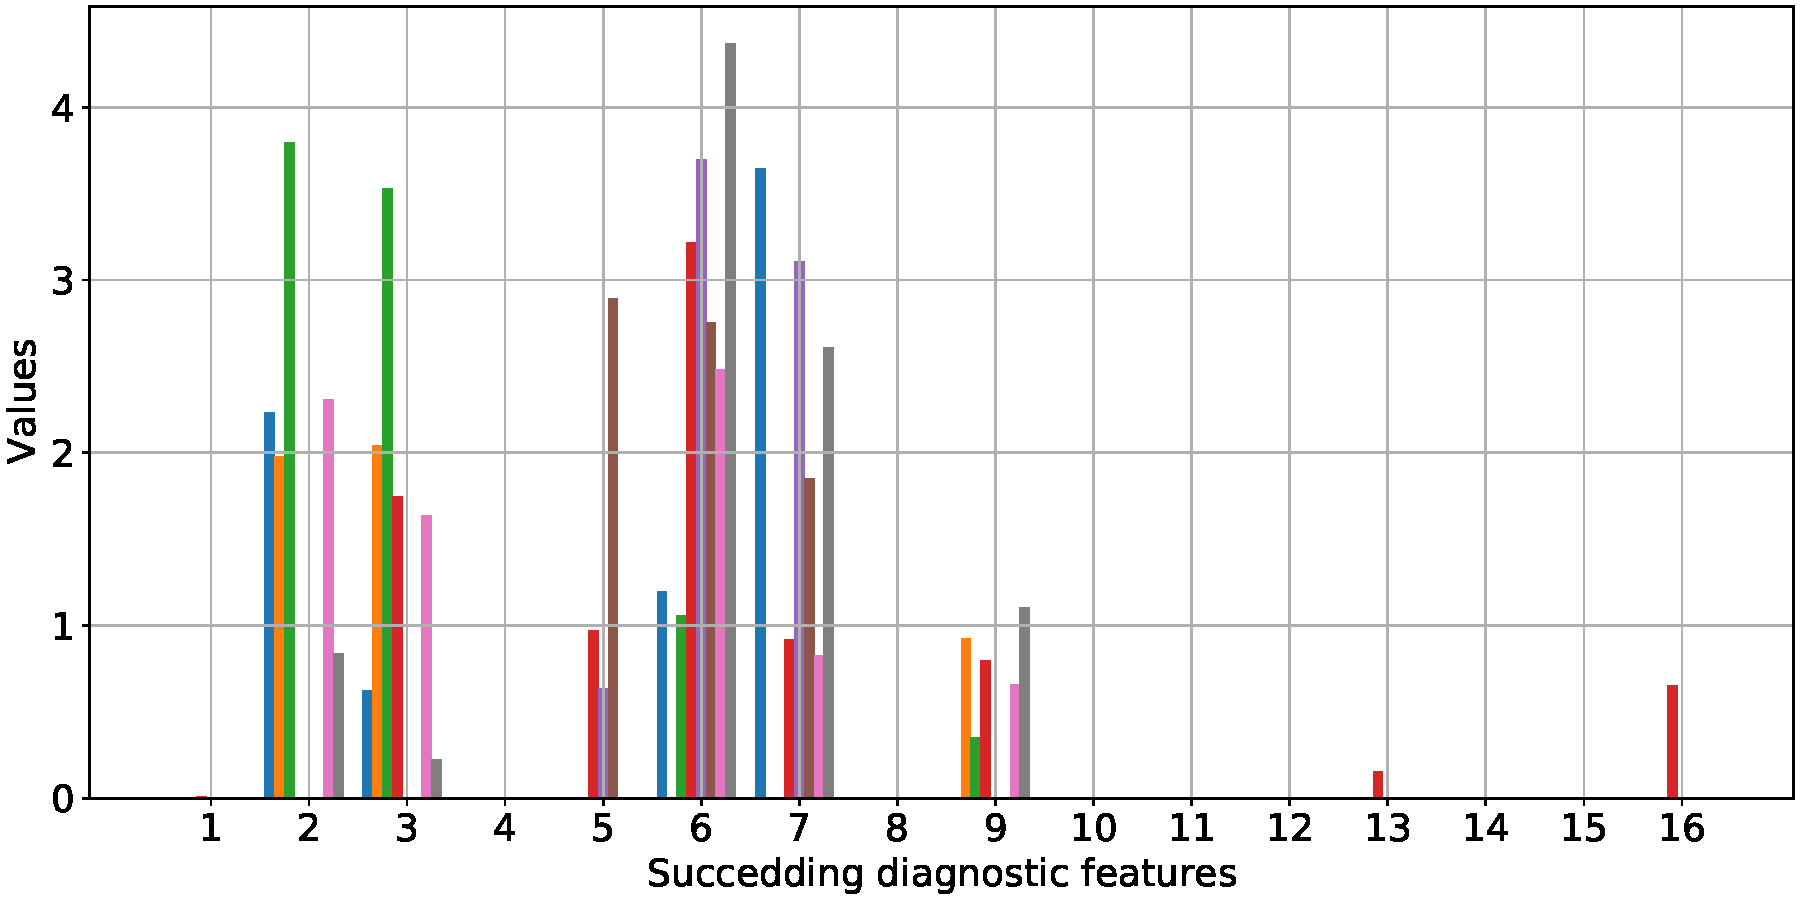
\includegraphics[width=\columnwidth]{Encoderfeatures.pdf}
  \end{subfigure}

  \caption{The diagnostic feature representation of 8 different images of the same person: (above) the distribution of PCA feautes (below) the corresponding features created by an autoencoder}
  \label{features}
\end{figure}

For PCA, I have chosen a reduction to 150 principal components, which referring
\cite{abdi2007singular} gives a compression ratio of:

\begin{equation}
  1 - \frac{15 \times (1+192+168)}{192 \times 168} = 83.2\%
\end{equation}

and captures 55.1\% of variance as defined in Eq. (\ref{eq:energy}). The amount
DeepFace model generates 4096 features. As seen in
\cite{ramaiah2015illumination}, which merely employs 240 features to classify
the same dataset, one certainly does not need to use the entirety of 4096
features. However, to directly apply the DeepFace model to our problem, I will
use the full set of 4096 features for experimentation. 

Fig. \ref{features} illustrates the representation of the first 16 features
extracted by the two methods respectively. All of them correspond to eight
different images of the same person. The key to successful FR is insensitivity
of the extracted features to different poses and lighting conditions of the
face. The autoencoding principle to feature generation is very efficient in this
respect. This is seen well in Fig. \ref{features}: the activations of PCA
features fluctuate a lot. Values are positive and negative for the same person,
resulting in  high variance. In contrast, the features computed by the
autoencoder are around the same level for the same person. Note that because
only the first 16 features are shown, some signals are not or not fully
activated. Similar results are found in \cite{siwek2017autoencoder}, where the
authors show that autoencoders find better balanced discriminant features. The
different quality of encodings generated by the two approaches, can be caused
through the inherent limits, resulting from PCA only being a linear
transformation. Autoencoders on the other hand, introduce various
non-linearities, enabling it to find discriminant features a PCA simply cannot.
However, conventional autoencoder's transformation in a ``latent space'' are
relatively non intuitive as and thus functions more like a black box.
Nevertheless, our autoencoder is an CNN and as such consists of filters which
have an interpretable meaning. As illustrated in Fig. \ref{eigenfaces}, the PCA
obtains principal components which have very intuitive interpretations as
eigenfaces.

For face classification on the Yale Face Database, it was split at random choice
of learning and testing data, while maintaining 38 classes present in both
subsets respectively. 60\% of samples have been used in learning and 40\% in
testing. In the case of PCA, the classifier used is a SVM with Gaussian kernel.
The width of Gaussian function and regularization constant C have been adjusted
using \textit{GridSearchCV} employing a standard 5-fold cross validation applied
on the training set. Their optimal values found in experiments were as follows:
$C=1000$ and $\gamma=0.01$. In the case of the autoencoder, the softmax
classifier was trained for 50 epochs during each the model's performance was
validated on the crossentropy loss and weights optimized with ADAM.

The experimentation has been repeated 10 times at random choice of learning and
testing data. The models' testing performance of classifying 38 individuals 
are presented in Table \ref{scores}. These data correspond to the samples not 
taking part in learning. The results of PCA and autoencoder applications have 
been obtained for the same data base \cite{yalefaceB}\cite{yalefaceBcropped} and
represent the average accuracy followed by standard deviation obtained in all 
runs.

\begin{table}[h]
  \caption{The average accuracy of face recognition for 38 classes of data (persons) obtained at application of autoencoder and pca preprocessing}
  \begin{center}
  \begin{tabular}{|c|c|c|}
  \hline
  \textbf{Metric} & \textbf{PCA} & \textbf{Autoencoder} \\
  \hline
  Accuracy & 92.60\%$\pm$0.99\% & 94.94\%$\pm$0.50\%\\
  \hline
  \end{tabular}
  \label{scores}
  \end{center}
\end{table}

As expected, higher quality features result in better general FR performance.
Note that although the autoencoder has not been trained on the Yale Face Dataset
at all, it still managed to outperform the PCA. This suggests that underlying
filters of the CNN have successfully found encodings of human faces. To further
enhance the autoencoder's accuracy, one could train it with the actual dataset
instead. For qualitative evaluation of the two approaches, the first 12 images
and the classification result of the test set on one run are included in
appendix Fig. \ref{appendix:PCAgallery} and Fig. \ref{appendix:Encodergallery}.
PCA fails at recognizing very dark pictures, humans would not even be able to
distinguish a person from. On the other hand, the autoencoder was able
recognizing these aforementioned dark images.

\begin{figure}[h]
  \centering
  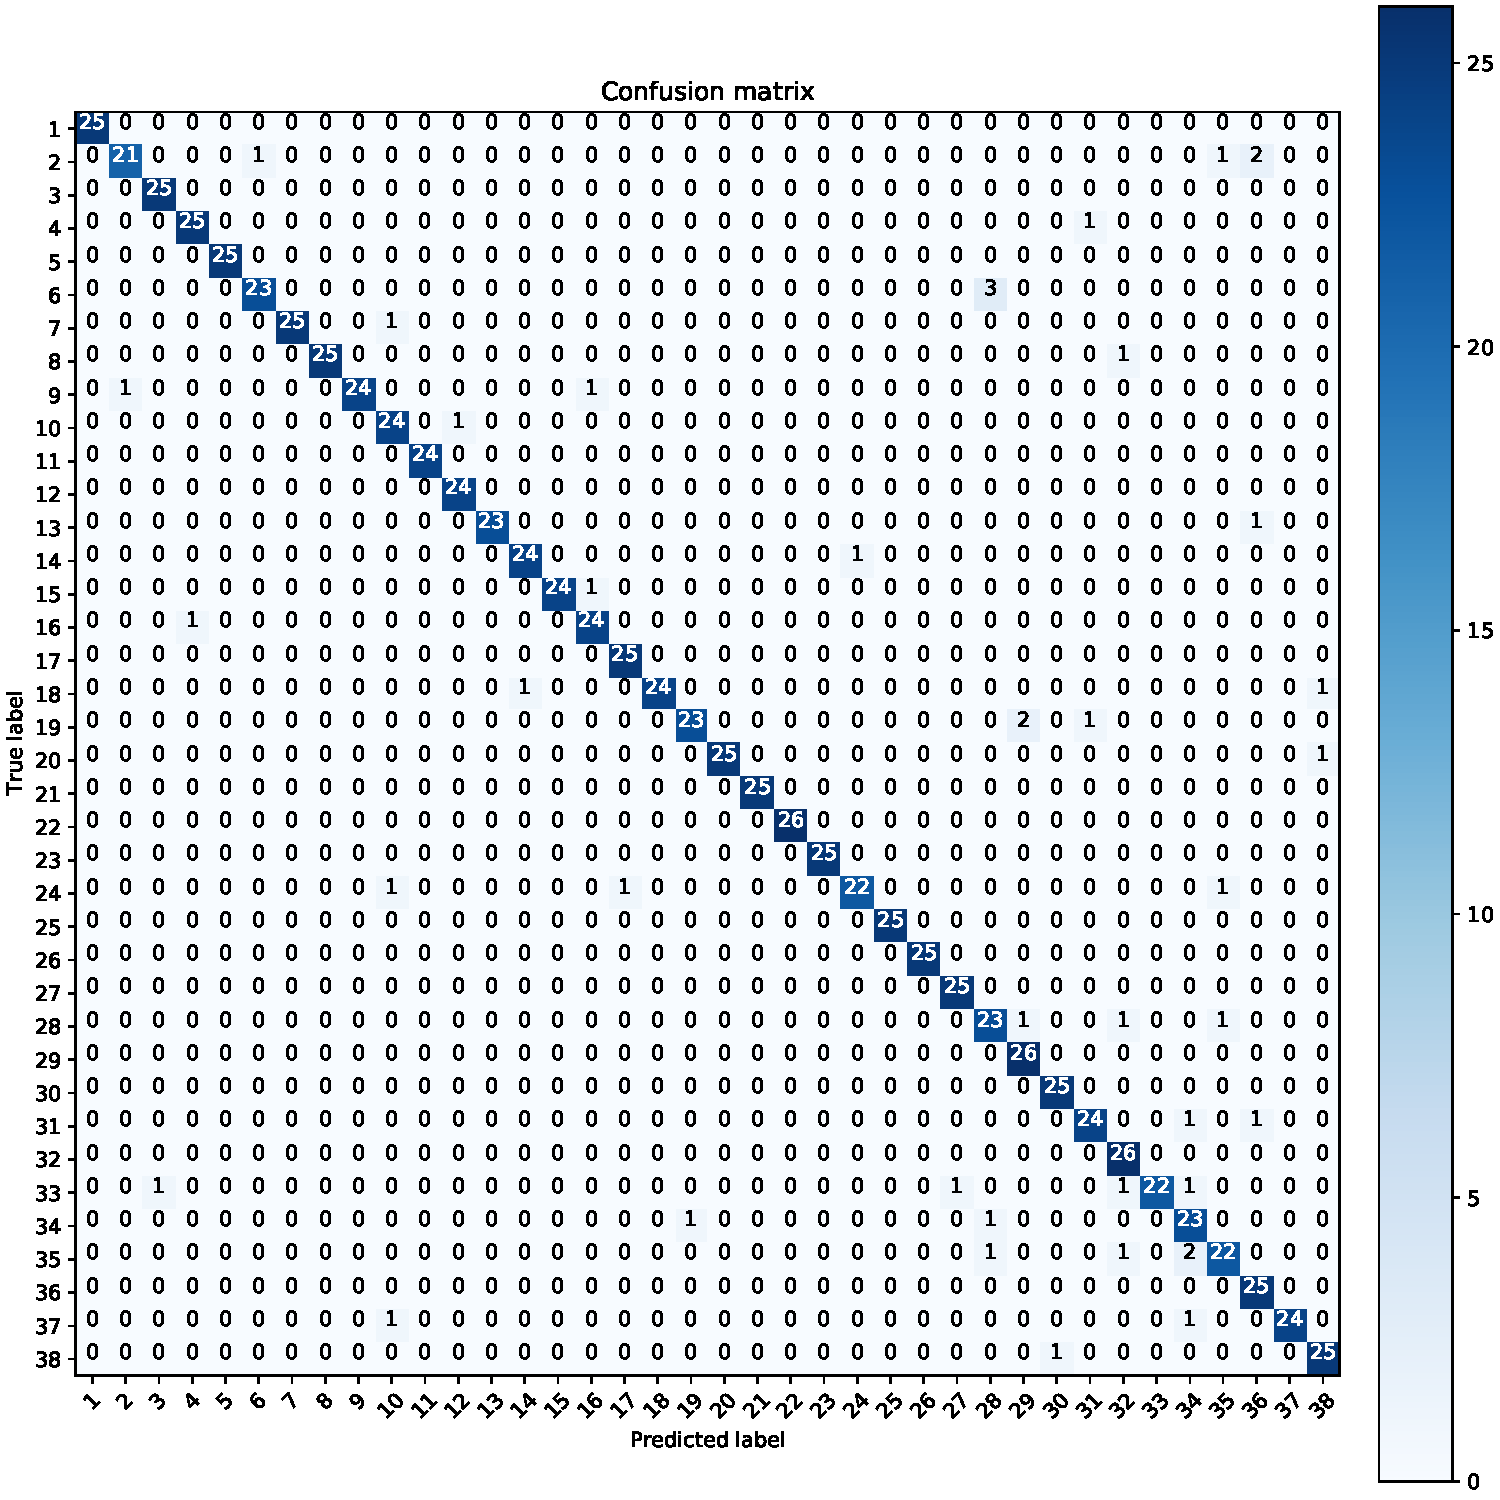
\includegraphics[width=\columnwidth]{EncoderConfusion.pdf}
  \caption{The confusion matrix of first 20 classes in face recognition at application of an autoencoder}
  \label{confusion}
\end{figure}

Fig. \ref{confusion} depicts the truncated confusion matrix after one run of the
autoencoder solution in recognition of 38 classes. For brevity, only the first
20 classes are plotted. We can see only scarce off-diagonal elements which are
different from zero. For comparison the full confusion matrix for PCA is
included in appendix Fig. \ref{appendix:PCAconfusion}.
